\documentclass{article}
\usepackage[utf8]{inputenc}
\usepackage[spanish]{babel}
\usepackage{graphicx}
\usepackage{caratula}
\usepackage[numbib,nottoc]{tocbibind}
\usepackage{csquotes}
\usepackage{biblatex}
\usepackage{amsmath}
\usepackage[spanish,onelanguage]{algorithm2e}

\addbibresource{informe.bib}

\materia{Laboratorio de Métodos Numéricos}
\titulo{Trabajo Práctico 1}
\subtitulo{Soda Stereo}

%\grupo{Grupo 12}
\integrante{Hosen, Federico}{825/12}{federico.hosen@gmail.com}
\integrante{Palladino, Julián Alberto}{336/13}{julianpalladino@hotmail.com}
\integrante{Rajngewerc, Guido}{379/12}{guido.raj@gmail.com}
\integrante{Silvani, Damián Emiliano}{658/06}{dsilvani@gmail.com}

\abstracto{Acá va el \textit{abstract} del trabajo práctico.}

\palabraClave{key1}
\palabraClave{keyN}

\begin{document}

\maketitle
\tableofcontents
\clearpage

\section{Introducción}

% Contendrá una breve explicación de la base teórica que fundamenta los métodos involucrados en el trabajo, junto con los métodos mismos. No deben incluirse demostraciones de propiedades ni teoremas, ejemplos innecesarios, ni definiciones elementales (como por ejemplo la de matriz simétrica). En vez de definiciones básicas es conveniente citar ejemplos de bibliografı́a adecuada. Una cita vale más que mil palabras.

La fotometría estéreo es una técnica de reproducción tridimensional de objetos a partir de un conjunto de fotografías. El método permite calcular los vectores normales a la superficie de un objeto en cada píxel de la imagen, observando a éste bajo distintas condiciones de luz\cite{Woodham80}.

En este trabajo práctico, se implementó el procedimiento de calibración y reconstrucción del mapa de normales y de profundidad para un conjunto de imágenes de un objeto.  Los métodos numéricos empleados para resolver los sistemas de ecuaciones que la técnica plantea fueron \textit{eliminación Gaussiana}, \textit{factorización LU} con pivoteo parcial y \textit{factorización de Cholesky}.


\section{Desarrollo}

% Deben explicarse los métodos numéricos que utilizaron y su aplicación al problema concreto involucrado en el trabajo práctico. Se deben mencionar los pasos que siguieron para implementar los algoritmos, las dificultades que fueron encontrando y la descripción de cómo las fueron resolviendo. Explicar también cómo fueron planteadas y realizadas las mediciones experimentales. Los ensayos fallidos, hipótesis y conjeturas equivocadas, experimentos y métodos malogrados deben figurar en esta sección, con una breve explicación de los motivos de estas fallas (en caso de ser conocidas).

\subsection{Calibración}

Para el proceso de calibración se implementó un programa \texttt{calibrate} que toma como parámetros una ruta a un conjunto de imágenes RGB de tipo \texttt{ppm}.  Se espera que las imágenes representen una esfera de material no especular, con una fuente de luz con distintas direcciones de luz.  Además, una de las imágenes debe ser una máscara de la esfera.

En la calibración se estima la dirección de la fuente de luz para cada imagen.  Para lograr esto, primero se busca el reflejo especular de la esfera.  Dado que se asume que la esfera tiene un materia con superficie Lambertiana, el brillo sólo depende de la orientación de ésta con respecto a la fuente de la luz.

\subsubsection{Color a escala de grises}

La primera dificultad que se nos presentó fue la de trabajar con imágenes RGB.  Lo que necesitamos tanto para la calibración como para el cálculo de las normales es interpretar la intensidad de luz de cada píxel.  Primero se decidió tomar el promedio del valor de cada canal RGB.  Como alternativa, se calculó el \textit{luma}, un promedio ponderado entre los 3 valores, donde se tiene en cuenta la manera en la que el ojo humano percibe los colores\cite{BT709}. Sean $R, G, B$ los valores rojo, verde y azul respectivamente, $L$ es el luma y se define como:

$$
L = 0.2126 \times R + 0.7152 \times G + 0.0722 \times B
$$

\subsubsection{Estimación de dirección de luz y detección de reflejo especular}

Siendo la superficie Lambertiana, la cantidad de luz reflejada en una localidad de la superficie es proporcional al coseno del ángulo formado por la normal en ese punto y la fuente de luz incidente.  Si el brillo en un punto de la imagen es máximo, podemos asumir que el ángulo allí es muy pequeño (porque $cos(x) \rightarrow 1$ si $x \rightarrow 0$), con lo cual, la normal es una buena estimación del vector de dirección de luz.

Por otro lado, como el objeto usado en la calibración es una esfera, la normal de cualquier punto de la superficie es conocida, y está dada por la ecuación de la esfera:

\begin{align*}
    x^2 + y^2 + z^2 &= r^2 \\
    \Rightarrow |z| &= \sqrt{r^2 - x^2 - y^2}
\end{align*}

Entonces, la dirección de luz incidente se puede estimar tomando el opuesto a la normal en el punto de mayor brillo.

Nuestro primer intento para encontrar el punto de mayor brillo en la esfera fue buscar el máximo valor en la matriz. ...

Para calcular el centro y el radio de la esfera se utilizó la máscara, porque la imagen tiene sólo dos colores y resulta más facil encontrar el \textit{bounding box} de la esfera.  A partir de éste, el centro y radio son fáciles de obtener.  Luego, la normal $n = (n_x, n_y, n_z)$ está dada por:

\begin{align*}
    n_x &= p_x - c_x \\
    n_y &= p_y - c_y \\
    n_z &= \sqrt{r^2 - p_x^2 - p_y^2}
\end{align*}

y por lo tanto, $l = -n$ es el vector de dirección de luz.

%\subsubsection{Pseudocódigo}
%
%\begin{algorithm}[H]
%\SetAlgoLined
%\KwResult{Write here the result }
% initialization\;
% \While{While condition}{
%  instructions\;
%  \eIf{condition}{
%   instructions1\;
%   instructions2\;
%   }{
%   instructions3\;
%  }
% }
% \caption{How to write algorithms}
%\end{algorithm}

\subsection{Reconstrucción 3D}

\subsubsection{Pseudocódigo}

\begin{algorithm}[H]
\SetAlgoLined
\KwResult{Matriz $N$ de normales para cada píxel}
  construir matriz $S$ a partir de $s_1$, $s_2$, $s_3$\;
  hacer factorización $LU$ de $S$\;
  \For{cada píxel $(x, y)$}{
    armar vector $I$ de los valores en $(x, y)$\;
    resolver sistema $Lx = I$ con EG\;
    resolver sistema $Um = x$ con EG\;
    $N_{x,y} = \frac{m}{\lVert m \rVert}$\;
  }
  \caption{Cálculo de normales}
\end{algorithm}

% TODO Estimación de la profundidad

\section{Resultados}

% Deben incluir los resultados de los experimentos, utilizando el formato más adecuado para su presentación. Deberán especificar claramente a qué experiencia corresponde cada resultado. No se incluirán aquí corridas de máquina.

% Ejemplo de figura gnuplot
\begin{figure}[ht!]
  \centering
  % GNUPLOT: LaTeX picture with Postscript
\begingroup
  % Encoding inside the plot.  In the header of your document, this encoding
  % should to defined, e.g., by using
  % \usepackage[latin1,<other encodings>]{inputenc}
  \inputencoding{latin1}%
  \makeatletter
  \providecommand\color[2][]{%
    \GenericError{(gnuplot) \space\space\space\@spaces}{%
      Package color not loaded in conjunction with
      terminal option `colourtext'%
    }{See the gnuplot documentation for explanation.%
    }{Either use 'blacktext' in gnuplot or load the package
      color.sty in LaTeX.}%
    \renewcommand\color[2][]{}%
  }%
  \providecommand\includegraphics[2][]{%
    \GenericError{(gnuplot) \space\space\space\@spaces}{%
      Package graphicx or graphics not loaded%
    }{See the gnuplot documentation for explanation.%
    }{The gnuplot epslatex terminal needs graphicx.sty or graphics.sty.}%
    \renewcommand\includegraphics[2][]{}%
  }%
  \providecommand\rotatebox[2]{#2}%
  \@ifundefined{ifGPcolor}{%
    \newif\ifGPcolor
    \GPcolortrue
  }{}%
  \@ifundefined{ifGPblacktext}{%
    \newif\ifGPblacktext
    \GPblacktexttrue
  }{}%
  % define a \g@addto@macro without @ in the name:
  \let\gplgaddtomacro\g@addto@macro
  % define empty templates for all commands taking text:
  \gdef\gplbacktext{}%
  \gdef\gplfronttext{}%
  \makeatother
  \ifGPblacktext
    % no textcolor at all
    \def\colorrgb#1{}%
    \def\colorgray#1{}%
  \else
    % gray or color?
    \ifGPcolor
      \def\colorrgb#1{\color[rgb]{#1}}%
      \def\colorgray#1{\color[gray]{#1}}%
      \expandafter\def\csname LTw\endcsname{\color{white}}%
      \expandafter\def\csname LTb\endcsname{\color{black}}%
      \expandafter\def\csname LTa\endcsname{\color{black}}%
      \expandafter\def\csname LT0\endcsname{\color[rgb]{1,0,0}}%
      \expandafter\def\csname LT1\endcsname{\color[rgb]{0,1,0}}%
      \expandafter\def\csname LT2\endcsname{\color[rgb]{0,0,1}}%
      \expandafter\def\csname LT3\endcsname{\color[rgb]{1,0,1}}%
      \expandafter\def\csname LT4\endcsname{\color[rgb]{0,1,1}}%
      \expandafter\def\csname LT5\endcsname{\color[rgb]{1,1,0}}%
      \expandafter\def\csname LT6\endcsname{\color[rgb]{0,0,0}}%
      \expandafter\def\csname LT7\endcsname{\color[rgb]{1,0.3,0}}%
      \expandafter\def\csname LT8\endcsname{\color[rgb]{0.5,0.5,0.5}}%
    \else
      % gray
      \def\colorrgb#1{\color{black}}%
      \def\colorgray#1{\color[gray]{#1}}%
      \expandafter\def\csname LTw\endcsname{\color{white}}%
      \expandafter\def\csname LTb\endcsname{\color{black}}%
      \expandafter\def\csname LTa\endcsname{\color{black}}%
      \expandafter\def\csname LT0\endcsname{\color{black}}%
      \expandafter\def\csname LT1\endcsname{\color{black}}%
      \expandafter\def\csname LT2\endcsname{\color{black}}%
      \expandafter\def\csname LT3\endcsname{\color{black}}%
      \expandafter\def\csname LT4\endcsname{\color{black}}%
      \expandafter\def\csname LT5\endcsname{\color{black}}%
      \expandafter\def\csname LT6\endcsname{\color{black}}%
      \expandafter\def\csname LT7\endcsname{\color{black}}%
      \expandafter\def\csname LT8\endcsname{\color{black}}%
    \fi
  \fi
  \setlength{\unitlength}{0.0500bp}%
  \begin{picture}(7200.00,4320.00)%
    \gplgaddtomacro\gplbacktext{%
      \csname LTb\endcsname%
      \put(561,372){\makebox(0,0)[r]{\strut{}-2.5}}%
      \csname LTb\endcsname%
      \put(561,840){\makebox(0,0)[r]{\strut{}-2}}%
      \csname LTb\endcsname%
      \put(561,1308){\makebox(0,0)[r]{\strut{}-1.5}}%
      \csname LTb\endcsname%
      \put(561,1776){\makebox(0,0)[r]{\strut{}-1}}%
      \csname LTb\endcsname%
      \put(561,2244){\makebox(0,0)[r]{\strut{}-0.5}}%
      \csname LTb\endcsname%
      \put(561,2711){\makebox(0,0)[r]{\strut{} 0}}%
      \csname LTb\endcsname%
      \put(561,3179){\makebox(0,0)[r]{\strut{} 0.5}}%
      \csname LTb\endcsname%
      \put(561,3647){\makebox(0,0)[r]{\strut{} 1}}%
      \csname LTb\endcsname%
      \put(561,4115){\makebox(0,0)[r]{\strut{} 1.5}}%
      \csname LTb\endcsname%
      \put(663,186){\makebox(0,0){\strut{}-30}}%
      \csname LTb\endcsname%
      \put(1909,186){\makebox(0,0){\strut{}-20}}%
      \csname LTb\endcsname%
      \put(3155,186){\makebox(0,0){\strut{}-10}}%
      \csname LTb\endcsname%
      \put(4401,186){\makebox(0,0){\strut{} 0}}%
      \csname LTb\endcsname%
      \put(5647,186){\makebox(0,0){\strut{} 10}}%
      \csname LTb\endcsname%
      \put(6893,186){\makebox(0,0){\strut{} 20}}%
    }%
    \gplgaddtomacro\gplfronttext{%
      \csname LTb\endcsname%
      \put(6105,3948){\makebox(0,0)[r]{\strut{}besj0(x)*0.12e1}}%
      \csname LTb\endcsname%
      \put(6105,3762){\makebox(0,0)[r]{\strut{}(x**besj0(x))-2.5}}%
    }%
    \gplbacktext
    \put(0,0){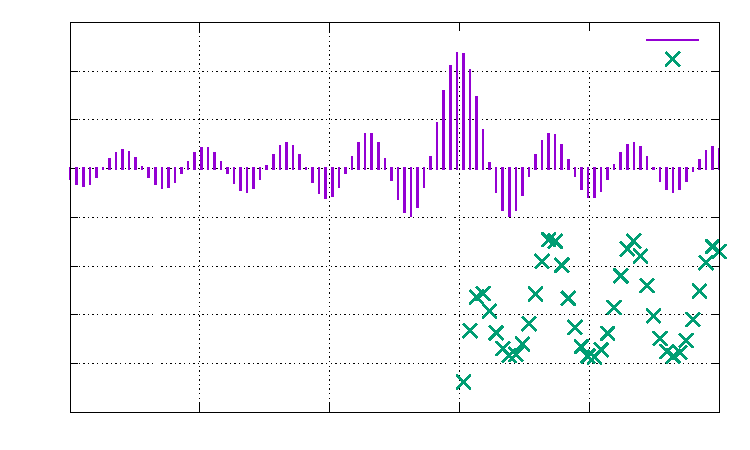
\includegraphics{plot/sample}}%
    \gplfronttext
  \end{picture}%
\endgroup

  \caption{Ejemplo de gnuplot, terminal cairo}
  \label{plot:}
\end{figure}


\section{Discusión}

% Se incluirá aquí un análisis de los resultados obtenidos en la sección anterior (se analizará su validez, coherencia, etc.). Deben analizarse como mínimo los ítems pedidos en el enunciado. No es aceptable decir que “los resultados fueron los esperados”, sin hacer clara referencia a la teoría la cual se ajustan. Además, se deben mencionar los resultados interesantes y los casos “patológicos” encontrados.

% Experimentos tentativos:
% Direcciones de luces:
% Que conversion de RGB a grises conviene utilizar? Promedio, promedio ponderado, norma 2(satura)
% (Puede cambiar el punto de mayor brillo con el que calibraremos?)
% Como cambia las luces obtenidas vs las luces de la catedra
% Ver como cambia la obtencion del mapa de normales (si no cambia demasiado en el resto del trabajo no incidira demasiado)
% 
% 
% Eleccion de luces como incide en el calculo de I0 y Ro.
% Se puede usar el numero de condicion para elegir la mejor combinacion de luces?
% El pixel elegido para obtener I0 y Ro incide en los valores obtenidos? Cuanto incide? Conviene tomar el mas brillante? Como elegirlo?
% 
% 
% Obtencion de normales
% Tiempos: Usar factorizacion Lu (O(n^3) + O(n^2.k)) vs usar EG clasico (O(n^3.k))
% Analizar la perdida de precision si se usa la suma de kahan o no (precision vs complejidad)
% ECG VS Pivoteo parcial vs pivoteo total
% Que optimizaciones podemos hacer sabiendo que la matriz es esparsa?
% 
% 





\section{Conclusión}

% Esta sección debe contener las conclusiones generales del trabajo. Se deben mencionar las relaciones de la discusión sobre las que se tiene certeza, junto con comentarios y observaciones generales aplicables a todo el proceso. Mencionar también posibles extensiones a los métodos, experimentos que hayan quedado pendientes, etc.


\clearpage
\section{Apéndices}

% En el apéndice A se incluirá el enunciado del TP. En el apéndice B se incluirán los códigos fuente de las funciones relevantes desde el punto de vista numérico. Resultados que valga la pena mencionar en el trabajo pero que sean demasiado específicos para aparecer en el cuerpo principal del trabajo podrán mencionarse en sucesivos apéndices rotulados con las letras mayúsculas del alfabeto romano. Por ejemplo: la demostración de una propiedad que aplican para optimizar el algoritmo que programaron para resolver un problema.


\clearpage
\printbibliography

% Es importante incluir referencias a libros, artículos y páginas de Internet consultados durante el desarrollo del trabajo, haciendo referencia a estos materiales a lo largo del informe. Se deben citar también las comunicaciones personales con otros grupos.


\end{document}
